\documentclass{article}

% if you need to pass options to natbib, use, e.g.:
%     \PassOptionsToPackage{numbers, compress}{natbib}
% before loading neurips_2021

% ready for submission
\usepackage[preprint]{neurips_2021}

% to compile a preprint version, e.g., for submission to arXiv, add add the
% [preprint] option:
%     \usepackage[preprint]{neurips_2021}

% to compile a camera-ready version, add the [final] option, e.g.:
%     \usepackage[final]{neurips_2021}

% to avoid loading the natbib package, add option nonatbib:
%    \usepackage[nonatbib]{neurips_2021}

\usepackage[utf8]{inputenc} % allow utf-8 input
\usepackage[T1]{fontenc}    % use 8-bit T1 fonts
\usepackage[colorlinks=true]{hyperref}       % hyperlinks
\usepackage{url}            % simple URL typesetting
\usepackage{booktabs}       % professional-quality tables
\usepackage{amsfonts}       % blackboard math symbols
\usepackage{nicefrac}       % compact symbols for 1/2, etc.
\usepackage{microtype}      % microtypography
\usepackage{xcolor}         % colors
\usepackage[backend=biber, sorting=none]{biblatex}
\addbibresource{references.bib}

% side by side figures
\usepackage{graphicx}
\usepackage{subfig}

\title{Assessment of Spotify Chart Preferences}

% The \author macro works with any number of authors. There are two commands
% used to separate the names and addresses of multiple authors: \And and \AND.
%
% Using \And between authors leaves it to LaTeX to determine where to break the
% lines. Using \AND forces a line break at that point. So, if LaTeX puts 3 of 4
% authors names on the first line, and the last on the second line, try using
% \AND instead of \And before the third author name.

\author{%
  Florian Kriegel\\
  Matrikelnummer 5746680\\
  \texttt{florian.kriegel@student.uni-tuebingen.de} \\
  \And
  Jonathan Währer\\
  Matrikelnummer 5776535\\
  \texttt{jonathan.waehrer@student.uni-tuebingen.de} \\\\\\
  github: \url{https://github.com/Fkrgl/Kriegl_Waehrer_spotify}
}

\begin{document}

\maketitle

\begin{abstract}
  In this project we aim to assess feature importance with regards to the popularity of a song. For this we collected a data set of all available top 50 charts playlist on spotify for different countries and applied dimensionality reduction (t-SNE) in combination with different coloring scales based on certain feature values. 
  Additionally, two regression models (linear and logistic) were trained with the goal to predict the popularity of a song based on the collected features and to classify whether a song of interest can deemed as \textit{chart material}.
\end{abstract}

\section{Introduction}
The music streaming platform Spotify is the most popular music streaming service nowadays. With over 381 million users, it provides a sound representation of today's most successful songs \cite{Spotify_users}. 
Thus, song data from Spotify can be used to analyse features of the currently most popular songs from all around the world. Spotify provides his own popularity measure to access song popularity based on play frequency and currentness \cite{Spotify_pop}.\\
In this report, we aim to identify important features for song popularity and use them to predict song popularity. For this, we acquired a data set of popular songs from the top 50 charts of all countries in spotify and a Kaggle dataset with 1.2+ million songs (not part of the charts).
Firstly, we used t-SNE to explore structure of the data. Next, linear and logistic regression models were trained to predict the popularity of a song based on pre-selected features.

\section{Materials and Methods}
\subsection{Data Acquisition}
In a first step, we downloaded the top 50 chart of 51 different countries from spotify as representative popular songs. 
For this, we used the spotify developer's API \cite{Spotify_developers} to download 20 meta and audio features for each song from the 51 chart playlists (see script \texttt{download\_spotify\_data.py}) resulting in a total of 2549 songs. 
In order to also consider unpopular songs, we downloaded a data set with 1.2+ million songs from Kaggle \cite{Spotify_Kaggle} (see script \texttt{download\_kaggle\_data.py}).

\subsection{Data pre-processing}
We extracted all audio features from our data sets and ended up with nine nominal and three categorical features for each track. 
Duplicated songs in the chart data set were removed and the nominal features were scaled using Z-score transformation resulting in 1060 unique chart songs. \\
We produced a balanced training set for regression and classification by randomly sampled 1000 songs from the Kaggle data set as examples for more unpopular songs.
Finally, both data sets were merged and labeled according to their source (charts or Kaggle) resulting in a training data set with 2060 tracks.

\subsection{Visual feature pattern analysis}
Feature distributions were analysed using density histograms. To reveal more complex structure in the training data, we combined t-SNE with a color scaling on different features. 

\subsection{Regression and classification}
A linear regression model was trained on two thirds of our data set. 
The performance of our model was accessed using the root mean squared error (RMSE) of a 5-fold cross validation on the training set and the test set. 
Further, a logistic regression model was trained to distinct between unpopular (popularity $\leq$ 50) and popular (popularity > 50) songs.

\section{Results}

\subsection{Visual feature pattern analysis}
Figure \ref{densities} shows that the chart data sets popularity distribution is shifted towards high popularity values while the popularity distribution of Kaggle songs is shifted towards lower values. The features \texit{duration}, \textit{instrumentalness}, \textit{liveness}, \textit{speachiness} and \textit{tempo} have a fairly similar distribution in both samples. 
Only the features \textit{danceability}, \textit{energy}, \textit{loundness} and \textit{valence} ('mood' of the song measured from zero for sad to one for happy \cite{Spotify_developers}) also show noticeable differences in their distribution.
Based on this observation, we decided to train our models in two batches: one for all features and one only for the four that differ most between the two groups (danceability, energy, loundness and valence).

\begin{figure}
    \centering
    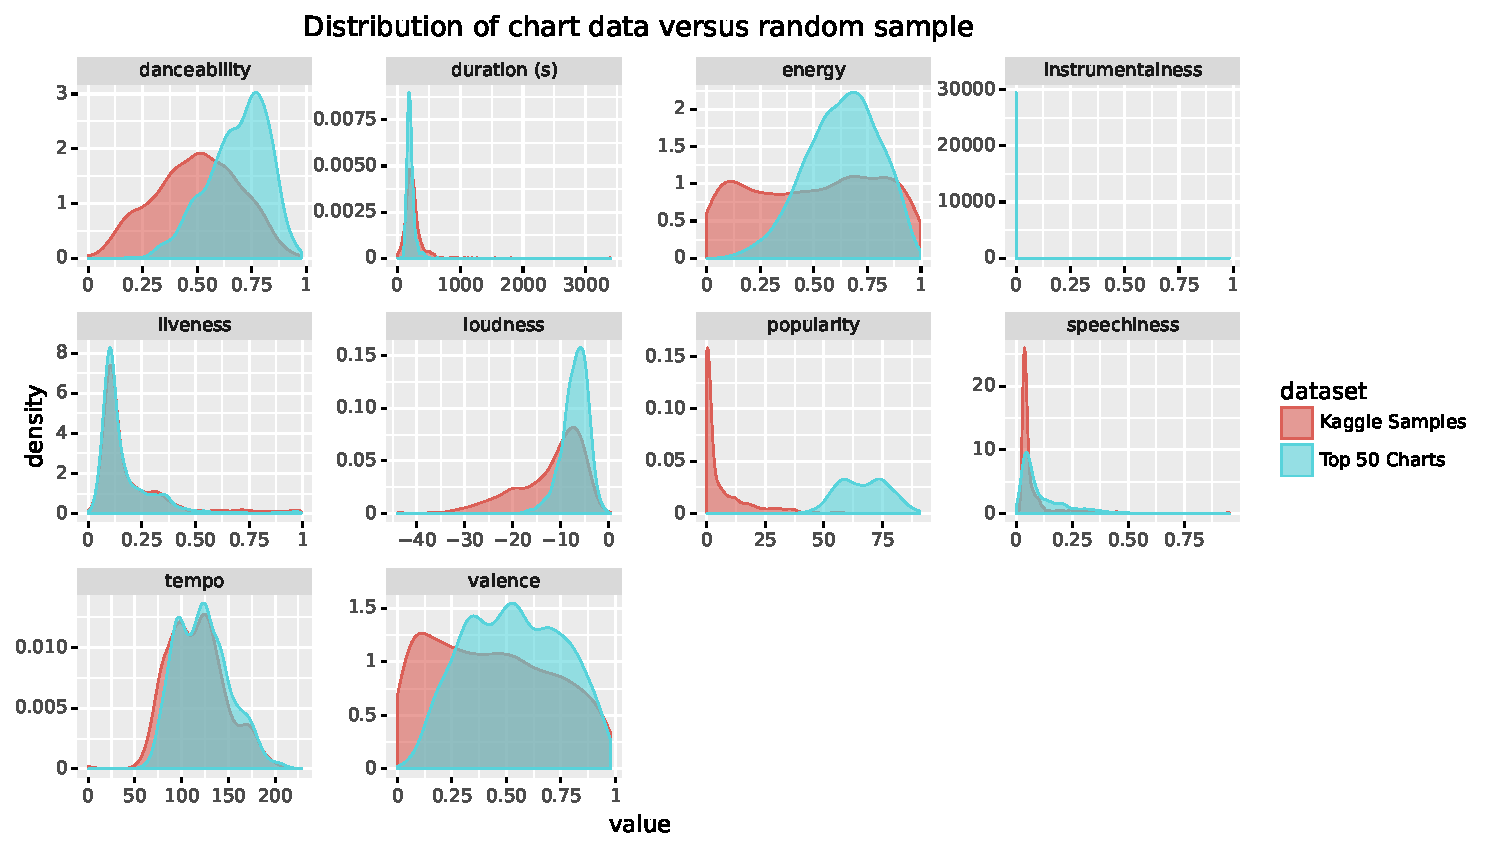
\includegraphics[width=0.9\textwidth]{code/fig/Charts_vs_random_samples.pdf}
    \caption{Distribution of selected features compared between chart and Kaggle data.}
    \label{densities}
\end{figure}

We analysed the four features using t-SNE and color coded each feature to highlight gradients in the produced map. Figure \ref{fig:f1} shows the t-SNE map on our training data color coded by the labels. Although, no distinct clusters become apparent, the color code reveals that chart tracks are over-represented in the lower right quadrant while the more unpopular kaggle tracks tend to cluster more in the top and left of the map. The color coding for the four most distinct features in figure \ref{fig:f2} show clear gradients in the t-SNE map. Here, we can see similar trends of the gradients of the features danceability and valence which show high values in the bottom left and low values towards the upper right. Thus, more danceable songs seem to also to be more happy and cheerful (high valence). Both, valence and danceability gradients roughly follow the popularity gradient indicating that popular songs tend to have higher values for both features compared to unpopular ones. Noticeably, a high energy measure can be found in both popular and unpopular songs. This can also be explained with the corresponding density histogram (figure \ref{densities}) and the uniform distribution of this measure for the Kaggle data set.

\begin{figure}[!h]
  \centering
  \subfloat[Colored by data source.]{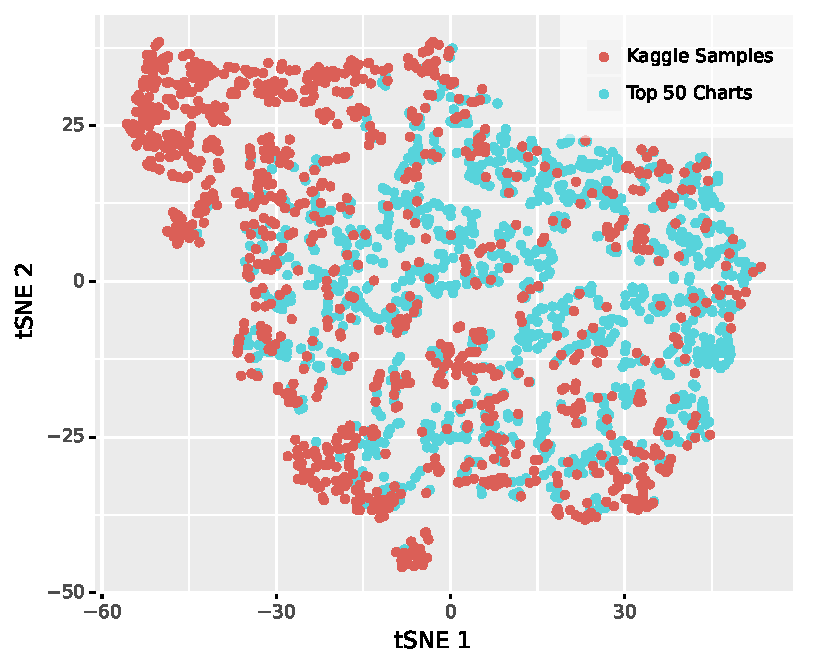
\includegraphics[width=0.4\textwidth]{code/fig/tSNE_datasets.pdf}\label{fig:f1}}
  %\hfill
  \subfloat[Colored by feature value.]{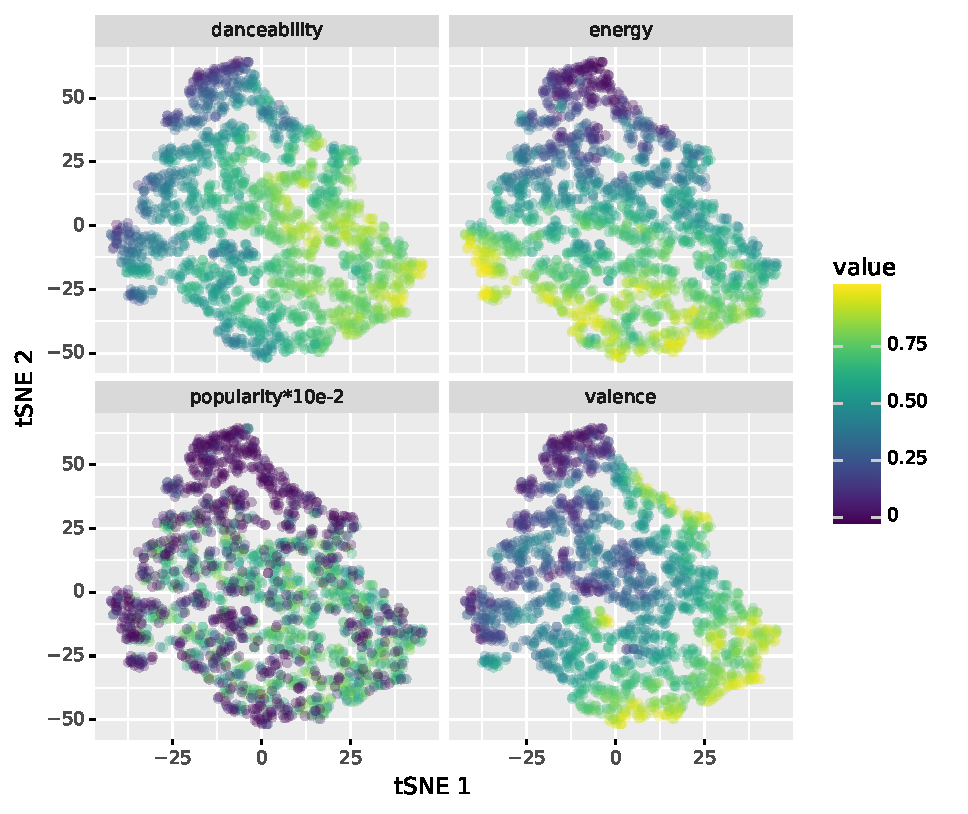
\includegraphics[width=0.4\textwidth]{code/fig/tSNE_features.pdf}\label{fig:f2}}
  \caption{Application of t-SNE to our data set with color coding corresponding to data set (a) or feature value for the most important features (b).}
\end{figure}

\subsection{Popularity prediction}

Figure \ref{performance} shows the performance of the linear and logistic regression models. For both models, the four most distinct features between the two groups achieved roughly the same performance compared to the models that used all 12 features. The residual plot for the linear regression model on four features in figure \ref{fig:f4} reveals a clear pattern in the residuals of the training data. Further, the color coding shows that our model seems to regard danceability as the most important indicator for song popularity because it tends to over predict songs with high danceability and underpredicts songs with low danceability. By taking the very different distributions between true and predicted popularity in figure \ref{fig:f5} into account, we conclude that the linear regression model is not capable of capturing the relationship between the features and the response. \\
According to the confusion matrix in figure \ref{fig:f6}, the logistic regression performs fairly well in distinguishing between popular and unpopular songs. 


\begin{table}
  \caption{Performance on test set for regression (RMSE) and classification (Accuracy) models} 
  \label{performance}
  \centering
  \begin{tabular}{lll}
  \\
    \toprule    
    model     & performance (12 features)     & performance (4 features) \\
    \midrule
    linear regression & 26.79  &   27.52   \\
    logistic regression & 0.78 &  0.75 \\
    \bottomrule
  \end{tabular}
\end{table}

\begin{figure}[!h]
  \centering
  \subfloat[Linear regression: Residual plot.]{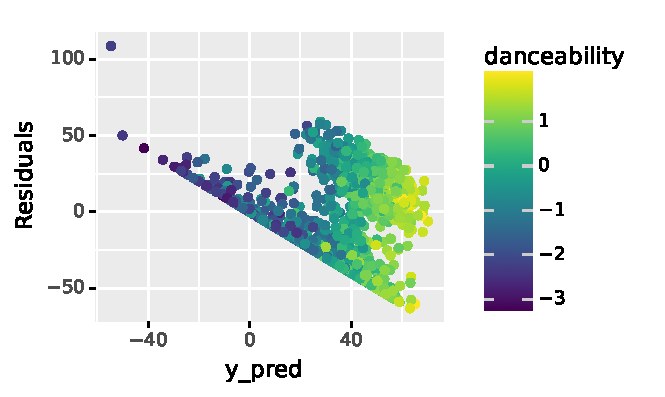
\includegraphics[width=0.5\textwidth]{code/fig/regression_residuals.pdf}\label{fig:f4}}
  %\hfill
  \subfloat[Linear regression: Popularity.]{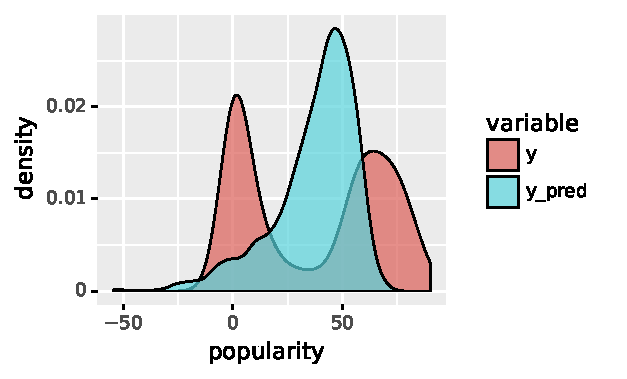
\includegraphics[width=0.5\textwidth]{code/fig/regression_true_vs_predicted.pdf}\label{fig:f5}}
  \hspace{0mm}
  \subfloat[Logistic regression: Confusion matrix.]{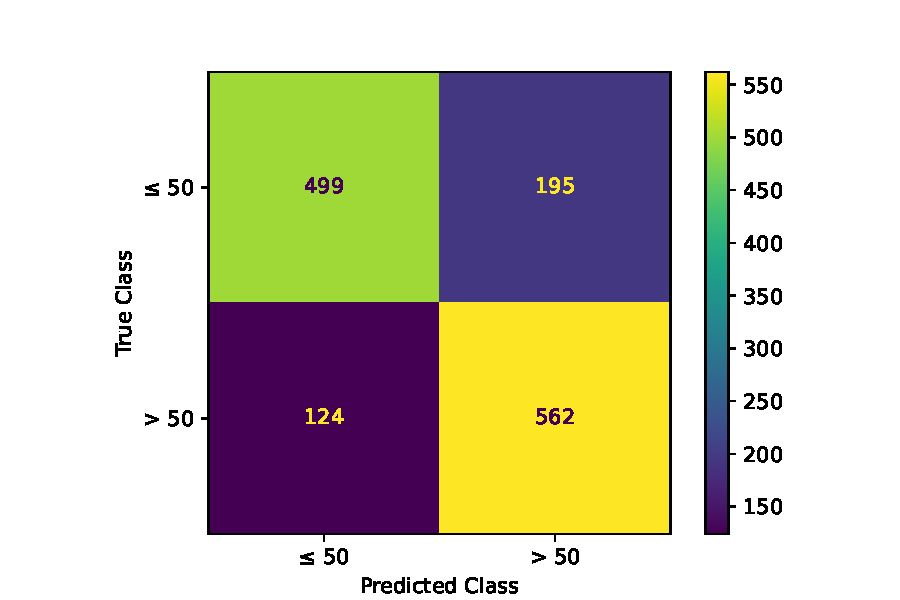
\includegraphics[width=0.6\textwidth]{code/fig/log_regression_confusion.pdf}\label{fig:f6}}
  \caption{Results of the logistic regression}
\end{figure}

\subsection{Discussion}
In this report, we aimed to analyse feature importance for the popularity measure of Spotify songs and used the results to train regression models to forecast song popularity.
Although, the visual feature pattern analysis revealed some differences in feature distributions between popular and unpopular songs, no distinct clusters tend to form in the t-SNE projections. We suggest that Especially songs with low popularity score but a high number of clicks cause problems here.\\
While we showed that logistic regression can be used in order to classify whether a song can be deemed as \texit{chart material}, other models have been applied for similar tasks and might be worth looking into \cite{araujo2020model}. 
It might also be possible to further improve our logistic regression model by extracting and analysing more features from the Spotify API or by adjusting the cutoff for the class assignation. 
An improvement could also achieved be by adjusting the popularity-cutoff: Based on the distribution of the popularity (figure \ref{densities}), the cutoff between the two data sets is slightly below 50 which might also improve our model. 
In conclusion, the aims of this project were partially fullfilled.
While there were no distinct t-SNE clusters, color-coding helped to somewhat assess the relationship between popularity and other features to a certain extend. What's more, while there is room for improvement on the statistical model, the results of this project have demonstrated the capability of simple models to predict the chart potential of a song with somewhat reasonable accuracy.

\section*{References}
\printbibliography[heading=none]


\newpage







\end{document}
